% !TeX root = ../main.tex

\chapter{预备知识与研究现状}\label{chap:background}

本章主要介绍强化学习的基本概念和一些预备理论知识,包括在Markov性质下使用动态规划求解最优决策策略的方法、使用策略梯度优化的方法近似求解最优策略的方法。随后介绍了使用经验样本回放和基于模型的强化学习的方法来提升样本利用效率、使用基于条件风险价值的样本筛选方法来提升策略鲁棒性。

\section{预备知识}

本节主要从强化学习的基本概念出发,对强化学习的问题背景和核心理念进行介绍,随后介绍强化学习算法中动态规划这一核心方法,最后介绍能衍生至深度强化学习算法的策略梯度优化方法。

\subsection{强化学习的基本概念}

强化学习算法的核心框架由智能体和环境信息构成,其中智能体指决策策略及其可观测的信息,环境则是全部信息空间中除智能体以外的所有信息。在强化学习中,环境和智能体都会随时间改变而变化,本文将指定时间下的环境信息集合定义为状态,而状态组成的集合定义为状态空间 $\mathcal S$ ,而在具体时刻 $t$ 的状态记作 $S_t\in \mathcal S$ 。本文将智能体在给定状态下能执行的决策行为定义为动作,将所有可执行的动作定义为动作空间$\mathcal{A}$,一般将给定状态 $S$ 和具体时刻 $t$下的动作记为 $A_t\in\mathcal{A}(s)$ 。

智能体执行 $A_t$ 后,环境信息集合会随之影响而发生改变,由当前状态 $S_t$ 转变为未来状态 $S_{t+1}$ 。在该转变过程中,环境还有一个反馈能力,可以根据动作$A_t$在自身中的表现反馈一个用于评价动作好坏程度的奖励指标 $R_{t}\in\mathcal{R}$ 。定义策略为映射关系:$\pi:\mathcal{S}\times\mathcal{A}\to \mathcal{P}$ ,其中$\mathcal P$表示整体概率空间。策略函数 $\pi(a|s)$ 表示智能体在面对状态 $S$ 时决策采取动作 $A$ 的概率。智能体根据反馈的奖励指标 $R_{t}$ ,可以调整自身策略中对应动作的概率系数,将高奖励反馈的动作赋予更大的执行概率,将低奖励反馈的动作赋予更低的执行概率,通过调整决策策略以使未来的决策动作能收到更好的奖励反馈。这样的策略调整过程称为策略学习或策略优化。在强化学习中,为了能够计算长期的收益,需要定义完整轨迹上的总收益,一般称这样的总收益为轨迹返回值,可如下所示定义 $t$ 时刻到结束时刻$T$的轨迹返回值 $G_t$ :
\begin{equation}
G_t = R_{t+1}+R_{t+2}+R_{t+3}+\cdots+R_T.
\end{equation}
对于无限长轨迹的强化学习问题问题,上述的返回值定义会趋于$\infty$,无法比较动作之间的差异,此时需要重新定义 $G_t$:
\begin{equation}
G_t = R_{t+1}+\gamma R_{t+2}+\gamma^2 R_{t+3}+\cdots = \sum_{k=0}^{\infty}\gamma^kR_{t+k+1}.
\end{equation}
其中 $\gamma(0\leq \gamma < 1)$ 为削减系数,通过不断累积削减系数,返回值将表现为更加关注近期时刻的奖励反馈。

在强化学习中,一般假定环境满足Markov性质,并将智能体与满足Markov性质的环境进行交互决策的过程称为Markov决策过程(Markov Decision Process,MDP)\cite{white1963dynamic,ross1996stochastic}。在MDP中,每一时刻的状态仅与前一时刻状态相关,与其他任意时刻的状态均无关。Markov性质的定义如下
\begin{definition}
设完整历史信息的联合概率分布为
\begin{equation}
    \mathrm{Pr}\{S_{t+1}=s',R_{t+1}=r|S_0,A_0,R_1,\ldots,R_t,S_t,A_t\}.
\end{equation}
设状态转移概率分布为
\begin{equation}
    p(s',r|,s,a) = \mathrm{Pr}\{S_{t+1}=s',R_{t+1}=r|S_t=s,A_t=a\}.
\end{equation}
当决策过程满足条件
\begin{equation}
  p(s',r|s,a) = \mathrm{Pr}\{S_{t+1}=s',R_{t+1}=r|S_0,A_0,R_1,\ldots,S_t,A_t\},
\end{equation}
称该决策过程具有Markov 性质。
\end{definition}

满足Markov性质的决策过程即为Markov决策过程\cite{sutton2018reinforcement,white1963dynamic}。在满Markov 决策过程中,智能体进行决策时仅需考虑当前时刻的状态信息集合。
此时可如式(\ref{eq:vbell})和(\ref{eq:qbell})定义状态价值函数和动作价值函数:
\begin{equation}\label{eq:vbell}
\begin{aligned}
    v_{\pi}(s)&=\mathbb{E}_{\pi}\left[G_t|S_t=s\right]\\
    &=\mathbb{E}_{\pi}\left[\sum_{k=0}^{\infty}\gamma^kR_{t+k+1}\mid S_t=s\right], \forall s \in \mathcal{S},
\end{aligned}
\end{equation}
\begin{equation}\label{eq:qbell}
\begin{aligned}
    q_{\pi}(s,a)&=\mathbb{E}_{\pi}\left[G_t|S_t=s,A_t=a\right]\\
    &=\mathbb{E}_{\pi}\left[\sum_{k=0}^{\infty}\gamma^kR_{t+k+1}\mid S_t=s,A_t=a\right].
\end{aligned}
\end{equation}
状态价值函数$v_\pi(s)$ 表示智能体以状态$s$为初始状态,通过策略函数 $\pi$ 与环境交互生成决策动作并执行,最终所能得到的轨迹回报值期望;行动价值函数 $q_\pi(s,a)$ 表示只能体以状态 $s$ 为初始状态,在确定执行动作 $a$后 ,通过策略函数 $\pi$ 与环境交互生成决策动作并执行,最终所能得到的轨迹回报值期望。

\subsection{动态规划求解最优策略}

强化学习算法的目标是求解Markov决策过程的最优策略,最优策略和其对应的价值函数定义如下
\begin{definition}
    在概率空间 $\mathcal{P}$ 中存在且至少存在一个策略优于其他所有策略,称满足这一条件的策略为最优策略,记作$\pi^*$,其对应的最优状态价值函数记为 $v_*(s)$,对应的最优动作价值函数记为 $q_*(s,a)$。
\end{definition}

而在有限Markov决策过程中,对于任意前后状态$s$和$s^\prime$,均存在Bellman 最优方程关系\cite{white1963dynamic}:
\begin{equation}\label{eq:v_star}
    v_*(s)=\max_{a}\sum_{s',r}p(s',r \mid s,a)[r+\gamma v_*(s')],
\end{equation}
\begin{equation}\label{eq:q_star}
q_*(s,a) = \sum_{s',r}p(s',r \mid s,a)\left[r+\gamma \max_{a'}q_*(s',a') \right].
\end{equation}

通过求解Bellman最优方差得到解 $v_*,q_*$ ,可进一步推导最优策略的形式,此时可将最优策略定义如下:
\begin{definition}
    记动作价值函数值能达到 $q_*$的动作为 $a_*$,如果一个策略$\pi$仅将非零概率赋予所有满足上述性质的$a_*$,称$\pi$为最优策略。
\end{definition}

基于以上定义可知,理论上求解 Bellman 最优方程即意味着解得最优策略,但由于Bellman方程难以直接求解且仅存在理论可解性,实际中需要使用动态规划的思想来迭代求解Bellman关系式以获取$v_*,q_*$的近似解\cite{sutton2018reinforcement}。在通过动态规划求解得到的价值函数之后,根据价值函数可优化更新决策策略$\pi$。策略优化算法的核心思路是按照如下公式选取最优动作$a$替换原有策略中的部分决策:
\begin{equation}
    \begin{aligned}
    \pi'(s) &= \mathop{\arg\max}\limits_a q_\pi(s, a)\\&=\mathop{\arg\max}\limits_a \mathbb{E}[R_{t+1}+\gamma v_\pi(S_{t+1})\mid S_t=s,A_t=a] \\&= \mathop{\arg\max}\limits_a \sum_{s',r} p(s', r | s, a) (r + \gamma v_\pi(s')).
    \end{aligned}
\end{equation}
具体的更新流程如算法~\ref{algo:bellman-update}~所示。将上述的值估计求解算法与策略优化算法相结合,进行循环优化,记策略价值函数估计(Policy Evaluation)为E步骤,由符号“$\xrightarrow{E}$”表示;记策略优化(Policy Improvement)为I步骤,由符号“$\xrightarrow{I}$”表示。则上述的循环优化过程可以表示为如式(\ref{process:EI})所示的流程:
\begin{equation}\label{process:EI}
\pi_0 \xrightarrow{E} v_{\pi_0} \xrightarrow{I}\pi_1 \xrightarrow{E} v_{\pi_1} \xrightarrow{I} \pi_2 \xrightarrow{E} \cdots \xrightarrow{I} \pi_* \xrightarrow{E} v_*
\end{equation}
通过循环优化过程,最终可以得到最终的收敛最优策略。

在有限Markov决策过程中,状态空间$\mathcal{S}$和行为动作空间$\mathcal{A}$都是有限的,显然可见策略空间也是有限的。而考虑到在策略价值函数估计和策略优化的循环过程中价值函数存在上界且单调递增,由单调收敛定理可知,存在一个步数$N$,当循环次数大于$N$后,所得策略能够近似逼近理想最优策略。

\begin{algorithm}[ht]
    \caption{基于 Bellman 迭代求解的强化学习算法}
    \label{algo:bellman-update}
    \begin{algorithmic}
        \STATE 初始化 $V(s), \forall s\in \mathcal S$
        \STATE 输入训练停止阈值$\delta$
        \STATE
        \REPEAT
        \STATE $\Delta= 0$
        \FOR{ $s\in\mathcal S$}
        \STATE $v= V(s)$
        \STATE $V(s)= \max_a\sum_{s',r}p(s',r|s,a)[r+\gamma V(s')]$
        \STATE $\Delta = \max(\Delta,|v-V(s)|)$
        \ENDFOR
        \UNTIL{ $\Delta<\delta$}
        \STATE $\pi(s)=\arg\max_a\sum_{s',r}p(s',r|s,a)[r+\gamma V(s')]$
        \STATE
        \STATE 输出最优策略 $\pi$
    \end{algorithmic}
\end{algorithm}

\subsection{策略梯度优化}

尽管动态规划算法能够理论上学习得到足够接近最优的策略,但直接求解的方法并没有充分发挥深度机器学习的优势。通过将策略函数进行参数化的做法,可以有效地结合机器学习中的梯度上升/下降算法,更为高效地进行策略学习\cite{sutton1999policy,grondman2012survey}。首先定义参数化的策略函数:
\begin{equation}
\pi ( a | s , \boldsymbol { \theta } ) = \operatorname { Pr } \left\{ A _ { t } = a | S _ { t } = s , \boldsymbol { \theta } _ { t } = \boldsymbol { \theta } \right\}.
\end{equation}
使用参数化决策策略所产生的价值函数,可定义参数化的性能目标函数:
\begin{equation}
    J(\boldsymbol{\theta}) \doteq v_{\pi_{\boldsymbol{\theta}}}\left(s_{0}\right),
\end{equation}
其中 $v_{\pi_{\boldsymbol{\theta}}}\left(s_{0}\right)$ 是 $\pi_\theta$ 初始状态为$s_0$条件下的真实价值函数 ,其中策略由 $\boldsymbol{\theta}$ 决定。通过对价值函数 $J ( \boldsymbol { \theta } )$ 的梯度进行梯度更新优化,可以实现性能的最优化,即
\begin{equation}
\boldsymbol { \theta } _ { t + 1 } = \boldsymbol { \theta } _ { t } + \alpha \widehat { \nabla J \left( \boldsymbol { \theta } _ { t } \right) },
\end{equation}
其中$\widehat { \nabla J \left( \boldsymbol { \theta } _ { t } \right) } \in \mathbb { R } ^ { d ^ { \prime } }$ 是梯度的估计值,满足$E_\boldsymbol{\theta}\left[\widehat { \nabla J \left( \boldsymbol { \theta } \right) }\right]=\nabla V(\boldsymbol{\theta})$,即其期望值为真实的梯度。基于以上的定义,可以给出如下定理:
\begin{theorem}
给定状态访问概率分布$\mu(s)$、行动价值函数$q_\pi(s,a)$,性能目标函数的梯度$\nabla J(\boldsymbol{\theta})$与策略函数的梯度$\pi(a | s, \boldsymbol{\theta})$存在如下所示的正比关系:
\begin{equation}
    \nabla J(\boldsymbol{\theta}) \propto \sum_{s} \mu(s) \sum_{a} q_{\pi}(s, a) \nabla \pi(a | s, \boldsymbol{\theta}),
\end{equation}
\end{theorem}
\begin{equation}
    \nabla J(\boldsymbol{\theta}) \propto \sum_{s} \mu(s) \sum_{a} q_{\pi}(s, a) \nabla \pi(a | s, \boldsymbol{\theta}).
\end{equation}
这一定理的意义在于,当直接优化目标函数的梯度$\nabla J(\boldsymbol{\theta})$时,等价于在对策略函数$\pi$进行梯度优化,即目标函数$J(\boldsymbol{\theta})$的最优化参数$\boldsymbol{\theta_*}$也是策略函数$\pi(a|s,\theta)$的最优化参数。在该定理的保证下,可以直接对$J(\boldsymbol{\theta})$进行简单的梯度优化即可求得最优策略。

\section{研究现状}

本节针对强化学习方法的样本利用效率问题和策略安全性问题,介绍现有工作中解决这两个问题的研究现状,主要分为经验样本回放方法、基于模型的强化学习方法和基于条件风险价值的样本筛选方法。

\subsection{经验样本回放方法}

在Q-Learning、SARSA\cite{watkins1992q,sutton2018reinforcement}等传统的强化学习算法中,环境交互样本往往只被使用一次后便被立即放弃,不再重复使用。由于其中的一些样本含有较高的学习价值,训练一次后即将其丢弃的做法会大幅降低强化学习算法的样本利用效率,基于这一考虑,经验回放的方法得以提出\cite{lin1992self},它将重要的经验存储在样本池中加以多次重复利用,使得智能体能够学习过去的经验\cite{adam2011experience}。不过经验回放也存在一些局限性,如果智能体所处环境随时间会发生变化,过去的经验将完全无助于实时的策略学习。DQN算法\cite{mnih2013playing}将经验回放机制与强化学习算法相结合,对经验回放的样本进行了随机化处理,保证了样本的独立同分布特性,从而解决了经验回放的局限性,在保证算法稳定性的同时做到了样本效率的提升。

尽管DQN算法中所使用的经验回放机制借由随机性改进做到了算法样本效率的优化,但是仍然较为局限。后续的工作提出,在样本池中按优先级进行经验回放的做法将会更加有效,这样的算法称为优先经验回放算法(Prioritized Experience Replay, PER)\cite{schaul2015prioritized}。PER算法能够给更重要的样本赋予更高的优先级,确保更有价值的经验得到更多的回放,从而起到了提升样本效率的效果。在PER算法中,最为理想的方法是计算智能体在样本池中的样本上学习的次数,被学习次数越少的样本,越应该被优先提供给智能体进行学习,然而学习次数这个指标实际上不容易取得。更可行的方案是使用时序差分误差来辅助计算样本池中的采样优先级,时序差分误差大的样本,意味着策略在该样本所处状态上的决策效果存在较大改进空间,同样可以被认为是更有高学习价值的经验样本\cite{tesauro1995temporal},因此需要为其分配更高的优先级进行学习。

实验可以证明,PER算法在诸多测试环境下均取得了大幅的优化改进。不过PER算法的一个缺点是因为修改了样本池中的经验分布,基于强化学习的理论分析可知,经验分布的变动将会导致智能体学习有偏差的策略,因此,PER算法还需要重要性采样(Importance Sampling)\cite{tokdar2010importance}和分布修正估计(Distribution Correction Estimation)\cite{lee2021optidice}等技术加以辅助,用以修正其带来的经验分布偏差。然而对于这一问题,现有的方法仍然有种种不足之处,例如重要性采样方法实际中难以准确计算分布偏差,而分布修正估计方法依赖大量的计算资源,代价高昂。

经验回放的样本选取过程是众多研究工作所关注的一大重点,但与此同时,经验回放样本池的设计也是影响经验回放方法效果的一个重要因素。相关工作已经证明,经验回放样本池的容量会对经验回放算法的效果产生显著影响,过大或过小的的样本池均可导致算法的效率大幅下降\cite{zhang2017deeper}。导致这一现象的原因主要是当经验回放样本池填充满后需要丢弃一部分历史经验,传统的做法是直接按存储时间来依次丢弃,一些工作提出,不同的丢弃方式也将影响经验回放算法的效率\cite{pieters2016q}。

经验回放样本池的另一大研究重点是其中的样本分布。考虑到强化学习对探索和利用机制的需求,如果样本池中的样本分布仅能覆盖实际样本分布中的一小部分,则很可能导致初期训练过拟合、策略脱离实际分布、灾难性遗忘等诸多问题。为了解决上述提到的问题,相关工作提出,更高频地使用最新样本即时覆盖旧样本,可以更有效地帮助智能体学习探索经验\cite{de2015importance}。此外,还可以根据样本的时序差分误差、状态空间占比、奖励反馈等多个指标进行优先级覆盖,从而得以从不同角度解决经验回放方法的缺点。

\subsection{基于模型的强化学习方法}

尽管经验回放方法通过重复利用现有样本的做法使得强化学习算法的样本利用效率得到一定程度的提升,但其提升程度并不明显,基于模型的强化学习算法是另一类可以有效提升样本利用效率的方法,它通过监督学习训练得到环境状态转移模型,以该模型为模拟环境大量且快速地生成模拟样本,能够辅助策略学习,加速策略的收敛。基于模型的强化学习基本框架最早在1991年提出 \cite{Sutton1991DynaReacting},它实际上是一种模块化的思路,可以应用到现有的各种无模型强化学习算法算法中(例如PPO ,TD3,SAC等算法 \cite{schulman2017proximal,haarnoja2018soft}),旨在高效地利用经验数据,提高学习效率以及数据利用效率。如图~\ref{fig:dyna-structure}~所示,基于模型的强化学习算法融合了规化、决策和学习的方法,在传统的无模型强化学习方法基础上,增加了模型学习$\longrightarrow$模型$\longrightarrow$模型规划的过程 \cite{lin1992self},通过经验数据学习得到一个环境的模型,然后使用模型进行模拟规划,生成模拟数据辅助强化学习进行策略优化更新。

\begin{figure}[tbh]
\centering
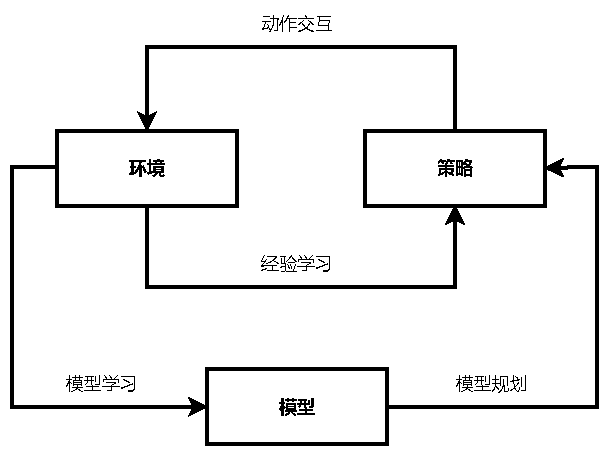
\includegraphics[width=0.8\textwidth]{figures/MBRL-struc.pdf}
\caption{基于模型的强化学习算法基本框架}
\label{fig:dyna-structure}
\end{figure}

在学得模型之后,最朴素的用法是,将真实环境数据和模型生成数据 混合,然后执行无模型强化学习方法,这一过程可视作一种数据增广的优化方法。更进阶的模型用法是,使用模型进行上下文信息的辅助计算,从而更高效地加速强化学习算法的收敛速度。虽然基于模型的强化学习算法有较好的样本效率,但由于模型误差,存在一定的局限性,使用这样有偏差的环境模型去预测,进而会带来更大的误差 \cite{zambaldi2018deep}。

在PILCO方法中 \cite{deisenroth2011pilco},通过学习环境的概率模型,从而实现对复杂环境的不确定性捕捉。具体地,PILCO方法使用了高斯过程回归模型来对环境建模 \cite{quinonero2005unifying},得到环境的概率模型$\mathcal{N}\left(\mu(s_t,a_t), \sigma(s_t,a_t)\right)$,基于这一概率模型,得到期望收益:
\begin{equation}
    J^\pi=\mathbb{E}_{s_{t+1}}\left[V\left(s_{t+1}\right)\right]=\int V\left(s_{t+1}\right) \mathcal{N}\left(s_{t+1} \mid \mu_t, \sigma_t\right) \mathrm{d} s_{t+1}.
\end{equation}
进而基于梯度$\dfrac{\mathrm{d}J}{\mathrm{d}\theta}$进行策略优化,得到最优参数,使得$\theta^* = {\arg\min}_\theta J^{\pi_\theta}$,最终训练得到最优策略$\pi^*=\pi_{\theta^*}$ 。\cite{peters2006policy}

不确定性环境模型将模型的误差以概率分布的形式展现出来,便能在模型的状态预测环节多次采样得到服从概率分布的预测状态,相比于传统的确定性预测模型,能够让强化学习策略更新环节接收到更多样化的样本输入,从而一定程度上抵消模型偏差带来的影响。但由于高斯过程回归并不适合对复杂的高维度环境进行建模,在后续的PETS方法\cite{Chua2018DeepModels}中,提出使用贝叶斯神经网络(BNN)来对复杂环境进行不确定性建模 \cite{Blundell2015WeightNetworks},从而解决了这一问题。如图~\ref{fig:BNN}~所示,贝叶斯神经网络的权重不再是固定的权值,而是一个概率分布,神经元间的权值将从这些概率分布中采样得到。

\begin{figure}[tbh]
\centering
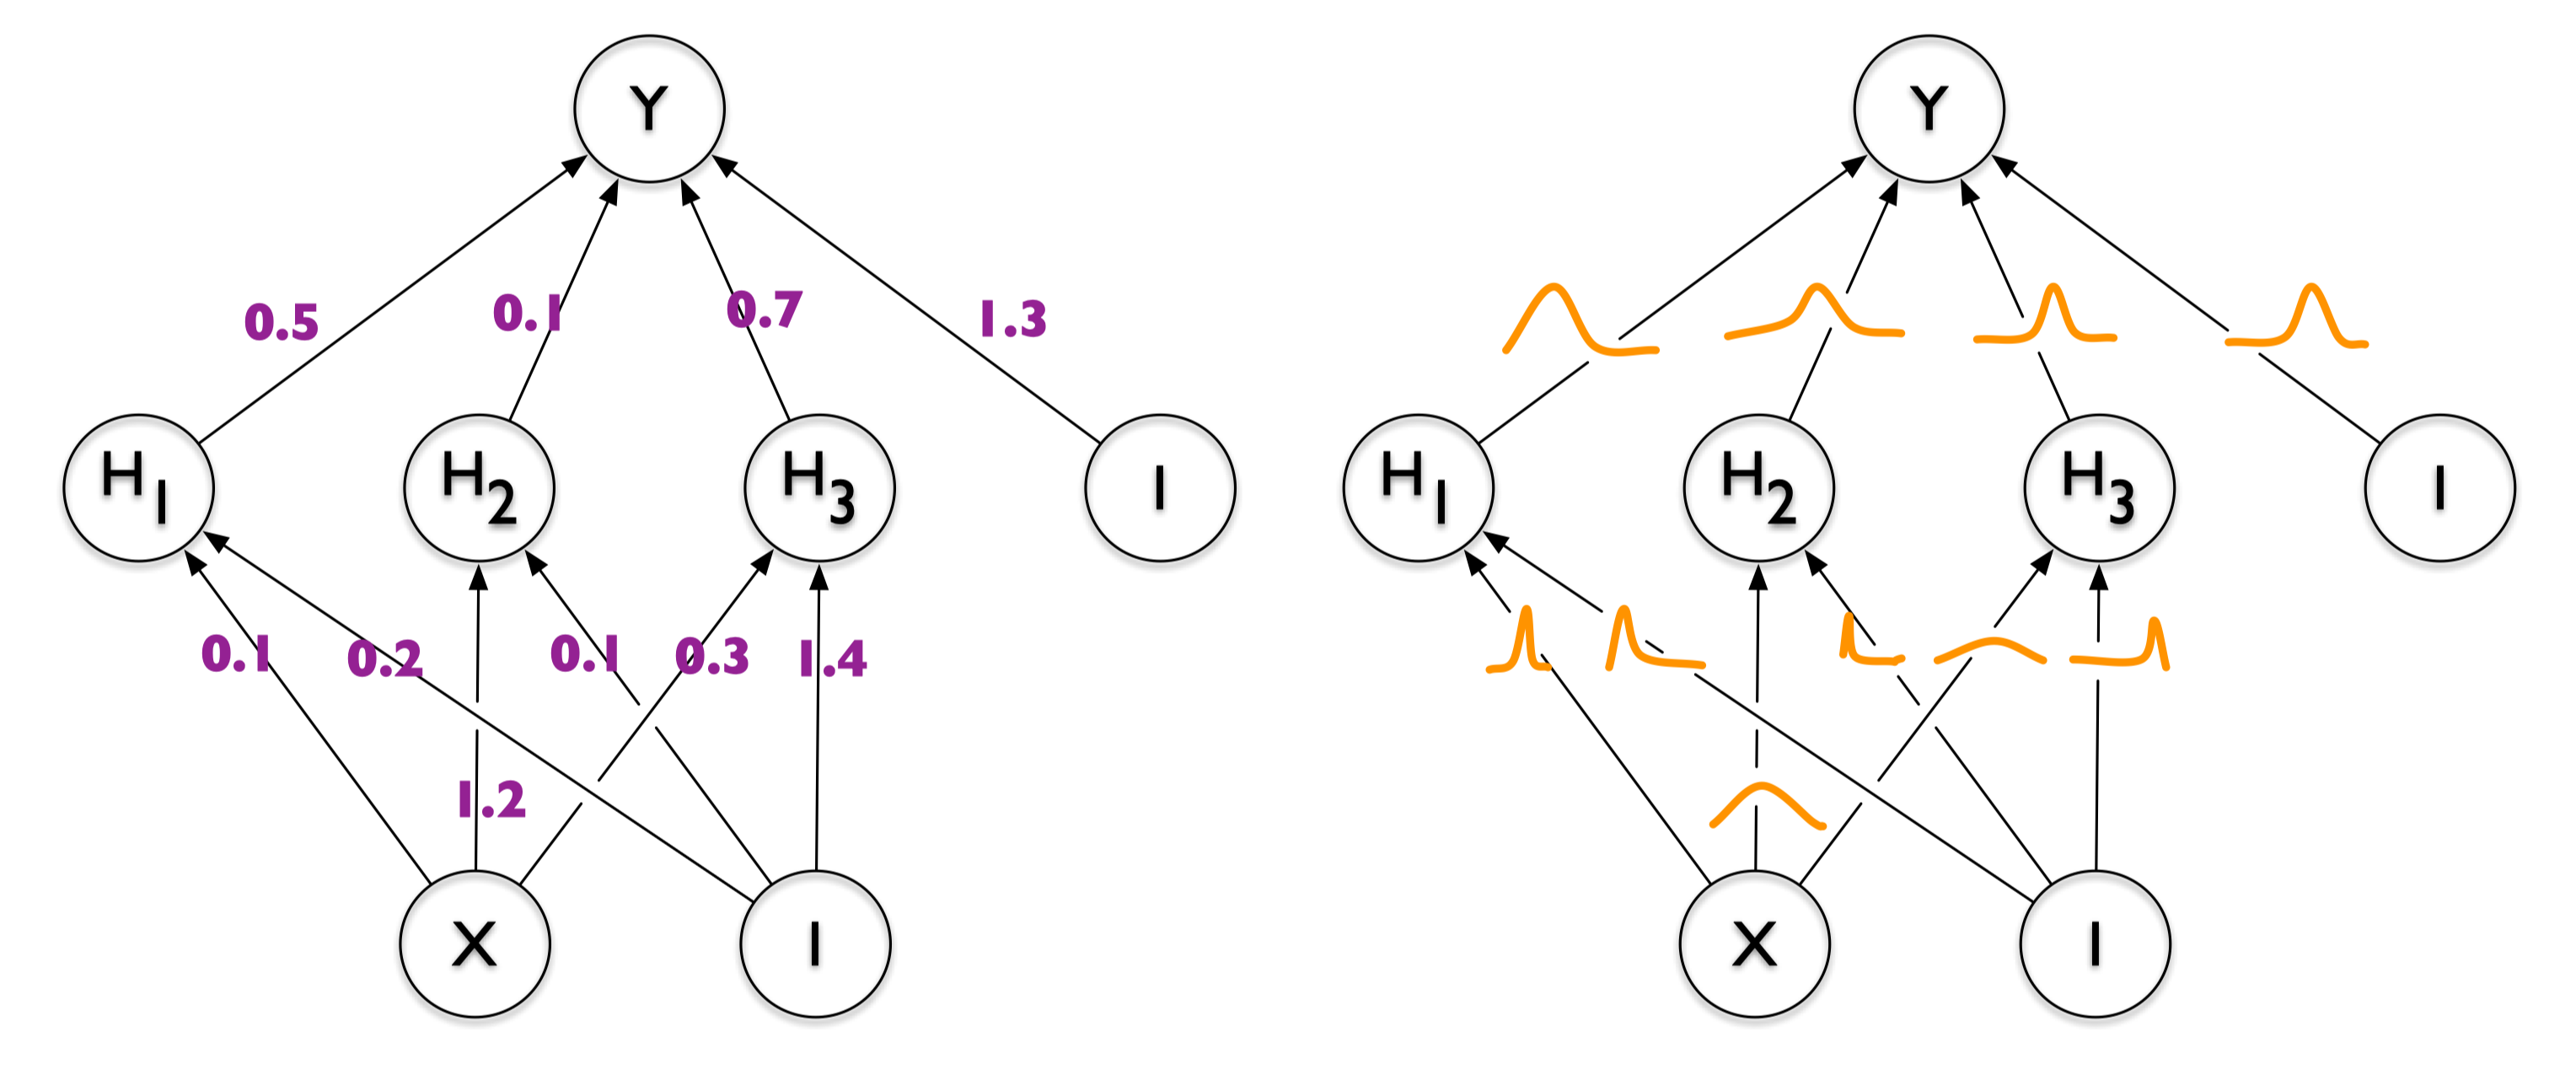
\includegraphics[width=0.9\textwidth]{figures/BNN.png}
\caption{贝叶斯神经网络与普通神经网络的区别示意图}
\label{fig:BNN}
\end{figure}

基于模型的强化学习另一大核心环节便是模型规划 \cite{walsh2010integrating},即使构建出一个准确的环境模型,如果不能合理地利用模型辅助强化学习,真实样本的利用效率依然无法得到提升。在MVE方法\cite{feinberg2018model}中 ,基于已构建的模型往后展开了$H$步的模拟。由于模型在当前时刻的未来较近步数有着较好的精准度,因此当$H$控制在一个合理范围下时,这$H$步的模拟累积误差相对传统的值函数估计要小很多,将这$H$步模拟替换掉值函数估计,便得到
\begin{equation}
    \widehat{V}_{H}\left(s_{0}\right)=\sum_{t=0}^{H-1} \gamma^{t} \hat{r}_{t}+\gamma^{H} \widehat{V}\left(\hat{s}_{H}\right).
\end{equation}

MVE将传统无模型强化学习中的值函数学习方法引入模型规划来辅助学习,采用了固定深度的模拟与对剩余部分估计的结合,实现了模型规划的优化。而在Re-Plan方法中 \cite{williams2017information},每次规划决策得到行动指令,并且基于该指令实际执行行动后,发现真实情况下的转移状态与之前模型规划得到的推理状态之间存在误差,该方法将真实状态进行储存,用作模型预测的修正,从而在下一次规划时,确保模型所预测的有误差状态能被存储记录修正,该方法可以有效地解决模型预测偏差的问题。

在MBPO方法中 \cite{janner2019trust},作者证明了当规划长度控制在一个可控长度$k$以内,即
\begin{equation}
k^{*}=\underset{k}{\operatorname{argmin}}\left[\frac{\gamma^{k+1} \epsilon_{\pi}}{(1-\gamma)^{2}}+\frac{\gamma^{k} \epsilon_{\pi}}{(1-\gamma)}+\frac{k}{1-\gamma}\left(\epsilon_{m^{\prime}}\right)\right]>0.
\end{equation}
此时,模型的误差始终可以保障在一个误差界限以内,从而在可控的预测误差下,能够最大程度地进行充分的模型规划预测。

\subsection{基于条件风险价值的样本筛选方法}

虽然目前基于模型的强化学习方法已经取得了显著的样本利用效率提升效果,但它们通常只适合于其所训练的环境,当部署到存在扰动的真实环境时,性能往往会急剧下降。

\begin{figure}
  \centering
  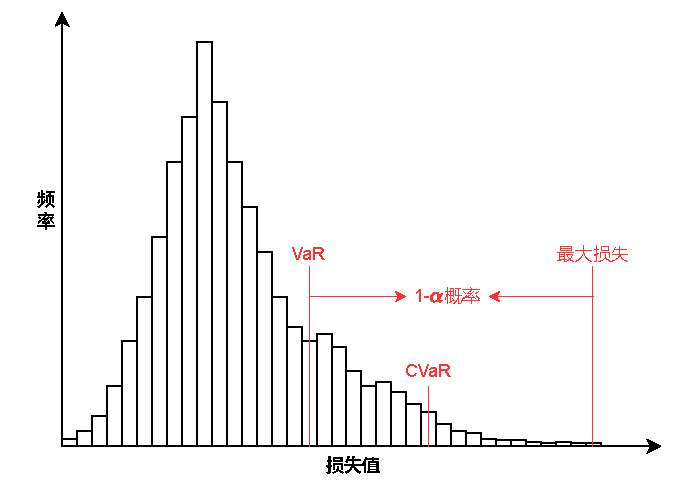
\includegraphics[width=\linewidth]{figures/CVaR.pdf}
  \caption{条件风险价值CVaR计算示意图}
  \label{fig:cvar}
\end{figure}

条件风险价值(CVaR)是一种用于计算最大风险的指标,如图~\ref{fig:cvar}~所示,首先需要定义风险价值(VaR)。记$Z$为随机变量,其累积分布函数为$F(z)=\mathrm{Pr}(Z<z)$,给定置信度$p \in (0,1)$,则关于 $Z$ 的$p$-置信度风险价值定义为$\mathrm{VaR}_p(Z)$:
\begin{equation}
\begin{aligned}
    \mathrm{VaR}_p(Z)&=F^{-1}(p)\\
    &\triangleq \inf\{z:F(z)\geq p\}.
\end{aligned}
\end{equation}
更进一步地,可定义条件风险价值(CVaR)。记关于$Z$的置信度$p$条件风险价值为$\mathrm{CVaR}_p(Z)$,其定义为关于随机变量$Z$的$p$百分比末尾分布期望值:
\begin{equation}\label{eq:def-cvar}
    \mathrm{CVaR}_p(Z)\triangleq \mathbb{E}[Z|Z\geq \mathrm{VaR}_p(Z)].
\end{equation}

CVaR的含义可解释为收益风险超过VaR部分的平均期望损失\cite{rockafellar2002conditional}。借由CVaR指标,可以通过学习消极样本数据来提高强化学习算法的鲁棒性,从而解决强化学习算法中安全性不足的挑战。

一些现有工作已经尝试以CVaR的思想,设计了样本筛选机制\cite{rajeswaran2016epopt},通过丢弃部分返回值更低的轨迹样本,适度抑制算法的学习速率,起到引导智能体更加关注低回报轨迹样本的作用,从而确保所学策略在面对异常状态时仍能保持较好的决策效果。实验表明,基于CVaR思想设计的样本筛选方法尽管可以一定程度地提升策略的整体稳定性和鲁棒性,但其也存在降低策略学习速度,减小样本利用效率等不足之处\cite{Tamar2015OptimizingSampling}。

\section{本章小结}

本章主要介绍了强化学习的基本概念,从基本的Markov性质及Markov决策过程出发,介绍了以Bellman方程为核心的动态规划求解方法,以及以梯度下降为核心的策略梯度优化方法等预备知识。并根据强化学习中样本效率问题及策略安全性问题的研究现状,介绍了经验样本回放方法,基于模型的强化学习和基于条件风险价值的筛选方法。